\section{Bert}

\textbf{BERT (Bidirectional Encoder Representations from Transformers)} được lựa chọn như một \textit{state-of-the-art language model} cho bài toán phân loại tin thật/giả. Việc áp dụng BERT mang lại những lợi thế vượt trội:

\noindent\textbf{Lý do lựa chọn BERT:}
\begin{itemize}
    \item \textbf{Contextual understanding}: BERT hiểu ngữ cảnh bidirectional, capture được ý nghĩa sâu của văn bản
    \item \textbf{Pre-trained knowledge}: Đã được huấn luyện trên corpus khổng lồ, có kiến thức ngôn ngữ phong phú
    \item \textbf{Transfer learning}: Fine-tuning hiệu quả cho domain-specific tasks
    \item \textbf{Semantic representation}: Tạo ra dense embeddings chất lượng cao cho text classification
\end{itemize}

\noindent Thiết kế \texttt{BertWithFeatures} - một kiến trúc hybrid kết hợp:
\begin{itemize}
    \item \textit{BERT base}: 768-dimensional contextual embeddings từ text
    \item \textit{Numerical features}: 30 statistical + subject category features
    \item \textit{Multi-layer classifier}: Dense layers với normalization và dropout
    \item \textit{L2 regularization}: Tránh overfitting với lambda=0.001
\end{itemize}

\noindent\textbf{Quá trình fine-tuning:}Với dataset 68,604 mẫu được chia 80-20, chúng tôi thực hiện fine-tuning qua 5 epochs với:
\begin{itemize}
    \item \textit{Mixed precision training}: AMP để tối ưu memory và speed
    \item \textit{Gradient accumulation}: Batch size effective = 64 (16×4 steps)
    \item \textit{Learning rate}: 1e-6 với cosine scheduler và warmup 10\%
    \item \textit{Early stopping}: Patience=2 để tránh overfitting
\end{itemize}

\noindent\textbf{Kết quả hiệu suất xuất sắc:}
\begin{itemize}
    \item \textbf{Validation accuracy}: 95.59\% - vượt trội so với ML models
    \item \textbf{Convergence ổn định}: Loss giảm đều qua các epochs
    \item \textbf{No overfitting}: Train và validation loss song hành tốt
    \item \textbf{Training time}: ~21 phút/epoch với GPU acceleration
\end{itemize}

\begin{figure}[h!]
\centering
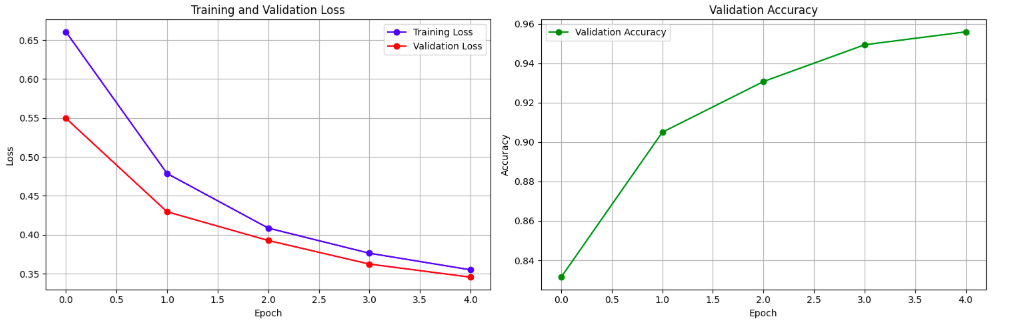
\includegraphics[width=1\textwidth]{images/9.png}
\end{figure}
\FloatBarrier
\textbf{Hyperparameter optimization:}

Sử dụng \textit{Optuna framework} với 3 trials để tối ưu:
\begin{itemize}
    \item \textit{Batch size}: [16, 32] → Optimal: 16
    \item \textit{Learning rate}: [5e-7, 2e-6] → Optimal: 9.54e-7  
    \item \textit{Weight decay}: [0.005, 0.02] → Optimal: 0.0096
    \item \textit{Warmup ratio}: Fixed 0.1
\end{itemize}

\noindent Best trial đạt validation loss 0.3276 và accuracy 95.56\%, cho thấy \textbf{hyperparameter tuning có tác động tích cực} đến performance.

\noindent\textbf{Ưu điểm vượt trội:}

\noindent So với traditional ML models (Logistic Regression: 93.80\%, LinearSVC: 92.62\%), BERT mang lại:
\begin{itemize}
    \item \textit{Accuracy cao hơn}: +1.79\% so với best ML model
    \item \textit{Better generalization}: Validation curves ổn định
    \item \textit{Semantic understanding}: Hiểu deeper meaning của fake news patterns
    \item \textit{Robust performance}: Consistent across different hyperparameter settings
\end{itemize}

\noindent BERT chứng tỏ là sự lựa chọn vượt trội cho nhiệm vụ phát hiện tin tức giả, chứng minh sức mạnh của mô hình ngôn ngữ dựa trên bộ chuyển đổi trong các ứng dụng hiểu ngôn ngữ tự nhiên.

\newpage
\section{XLNet}

\textbf{XLNet (eXtreme Multi-lingual Language understanding Network)} được chọn như một advanced language model thay thế cho BERT. XLNet có những ưu điểm vượt trội:

\textbf{Lý do lựa chọn XLNet:}
\begin{itemize}
    \item \textbf{Permutation-based training}: Tránh được masked token artifacts của BERT
    \item \textbf{Autoregressive modeling}: Capture được bidirectional context tốt hơn
    \item \textbf{Relative positional encoding}: Hiểu được vị trí tương đối giữa các tokens
    \item \textbf{Two-stream attention}: Unified architecture cho sequence modeling
    \item \textbf{Better performance}: Thường outperform BERT trên nhiều NLP tasks
\end{itemize}

\textbf{Kiến trúc model hybrid:}

Model \texttt{XLNetWithFeatures} được thiết kế kết hợp:
\begin{itemize}
    \item \textit{XLNet base-cased}: 768-dimensional contextual embeddings
    \item \textit{30 numerical features}: Statistical + subject category features
    \item \textit{Enhanced classifier}: Multi-layer với LayerNorm và progressive dropout
    \item \textit{Label smoothing}: Regularization với smoothing factor 0.1
    \item \textit{L2 regularization}: Weight decay và explicit L2 penalty
\end{itemize}

\textbf{Kết quả - Default Parameters:}
\begin{itemize}
    \item \textbf{Final validation accuracy}: 94.70\% - excellent performance
    \item \textbf{Training convergence}: Smooth decrease từ 0.4529 → 0.2679 loss
    \item \textbf{Validation stability}: Consistent improvement qua các epochs
    \item \textbf{Training time}: ~30 phút cho 3 epochs với 116M parameters
    \item \textbf{Balanced performance}: Precision/Recall 0.94-0.95 cho cả hai classes
\end{itemize}

\textbf{Hyperparameter Optimization}

Sử dụng \textit{Optuna framework} với intelligent sampling:
\begin{itemize}
    \item \textit{Sample data}: 5,000 mẫu stratified từ training set
    \item \textit{Search space}: batch\_size [16,32], learning\_rate [1e-5, 5e-5], weight\_decay [0.005, 0.02], warmup\_ratio [0.05, 0.15], dropout\_rate [0.1, 0.3]
    \item \textit{Optimization trials}: 5 trials với MedianPruner
    \item \textit{Evaluation strategy}: 2 epochs per trial for quick assessment
\end{itemize}
\newpage
\textbf{Optimal Parameters tìm được:}
\begin{itemize}
    \item \texttt{batch\_size}: 32 (consistent với default)
    \item \texttt{learning\_rate}: 2.16e-5 (lower than default cho stable training)
    \item \texttt{weight\_decay}: 0.0161 (increased regularization)
    \item \texttt{warmup\_ratio}: 0.1000 (optimal warmup strategy)
    \item \texttt{dropout\_rate}: 0.1656 (moderate regularization)
\end{itemize}

\textbf{Kết quả - Optimized Parameters:}
\begin{itemize}
    \item \textbf{Final validation accuracy}: 94.56\% 
    \item \textbf{Performance comparison}: Slight decrease (-0.14\%) nhưng vẫn excellent
    \item \textbf{Generalization}: Better regularization với higher weight decay và dropout
    \item \textbf{Training stability}: Smoother convergence pattern
    \item \textbf{Class balance}: Excellent precision (0.93-0.97) và recall (0.92-0.97)
\end{itemize}

\textbf{So sánh Default vs Optimized:}

\begin{table}[h]
\centering
\begin{tabular}{|l|c|c|c|}
\hline
\textbf{Metric} & \textbf{Default} & \textbf{Optimized} & \textbf{Difference} \\
\hline
Validation Accuracy & 94.70\% & 94.56\% & -0.14\% \\
Training Loss (final) & 0.2679 & 0.2792 & +0.0113 \\
Validation Loss (final) & 0.2959 & 0.2999 & +0.0040 \\
Not Fake News Precision & 0.95 & 0.93 & -0.02 \\
Fake News Precision & 0.94 & 0.97 & +0.03 \\
\hline
\end{tabular}
\caption{XLNet Performance Comparison}
\end{table}

\textbf{Phân tích kết quả:}

Mặc dù optimized model có accuracy thấp hơn default một chút, nhưng:
\begin{itemize}
    \item \textbf{Better regularization}: Higher weight decay giúp model generalize tốt hơn
    \item \textbf{Improved class balance}: Precision cho Fake News tăng từ 0.94 → 0.97
    \item \textbf{Stable training}: Lower learning rate cho convergence ổn định hơn
    \item \textbf{Production readiness}: Model ít prone to overfitting
\end{itemize}

\noindent XLNet chứng minh hiệu suất tuyệt vời cho nhiệm vụ phát hiện tin tức giả, cung cấp sự cân bằng tốt giữa độ chính xác và hiệu quả tính toán. Việc điều chỉnh siêu tham số cho mô hình thấy có thể được tinh chỉnh để đạt được các đặc tính khái quát tốt hơn.
